\documentclass{article}
\usepackage{amsmath, graphicx, amsfonts, caption, subfig, keyval, algorithm, algorithmic,xcolor}
\usepackage[margin=1in]{geometry}
\usepackage{setspace}
\usepackage{csquotes}

\captionsetup{justification=centering}
\newcommand{\R}{\mathbb{R}}
\newcommand{\Rr}{\mathcal{R}}
\newcommand{\D}{\mathcal{D}}
\newcommand{\C}{\mathcal{C}}
\newcommand{\X}{\mathcal{X}}
\DeclareMathOperator*{\argmin}{\arg\!\min}

\onehalfspacing

\begin{document}
\title{AM221 Final Project \\ \large Dictionary Selection Under a Supermodular Assumption}
\author{Taylor Killian \& Leonhard Spiegelberg}
\maketitle

\begin{abstract}
We attempt to develop a method by which to solve dictionary selection under a supermodular assumption. This method is motivated primarily by the work of Singer et al. (2016)~\cite{Singer16TwoStage} where a two-stage submodular maximization generalization was developed. The development of a two-stage supermodular minimization algorithm to address Sparse Dictionary Selection utilizes approximation results derived by Boutsidis et al. (2015)~\cite{weaklyalpha} for supermodular optimization. We show that Sparse Dictionary Selection is functionally equivalent to Sparse Multi Linear Regression which allows us to leverage~\cite{weaklyalpha}. We analyze and experiment with an implementation of our two-stage optimization routine and compare it to current methods. With this project we have laid the ground for further exploration into the formalization of the two-stage method that we propose here.
\end{abstract}

%%%%%%%%%%%%%%%%%%%%%%%%%%%%%%%%%%%%%%%%%%%%%%%%%%%%
%%-------------------------------                              Introduction                               -------------------------------%%
%%%%%%%%%%%%%%%%%%%%%%%%%%%%%%%%%%%%%%%%%%%%%%%%%%%%
\section{Introduction}\label{sec:intro}

Dictionary selection and sparse regression (problems that we show to be functionally equivalent) are variants of representation learning. The goal of these kinds of problems is to determine a sparse representation of input data in the form of a linear combination of basis elements as well as the basis elements themselves. That is, one essentially factors the input, or design matrix, into a sparse catalog and a dictionary of basis elements, both of which need to be inferred from the data.\\

%%%%%%%%%%%%%%%%
%%    Problem Definition     %%
%%%%%%%%%%%%%%%%
\subsection{Problem Definition}\label{sec:problem definition}
\noindent Dictionary learning, in its general form, can be seen as
\[
\min_{\D, \Rr, \theta, \lambda} f(\D, \Rr, X) + g(\D, \theta) + h(\Rr, \lambda)
\]
where $f$ describes the objective function used to measure goodness of approximation of $X$ through $\D, \Rr$, $g$ describing suitable constraints on the dictionary, $h$ on the representation respectively.\\

\noindent With an input dataset $X=[x_1, \dots, x_k],  x_i \in \R^d,  X \in \R^{d\times k}$ we wish to find a dictionary $\D \in \R^{d\times n}, \   \D~=~[d_1, \dots, d_n]$ and a representation $\Rr \in\R^{n\times k}, \ \Rr = [r_1,\dots,r_k], \ r_i\in\R^n $  such that both $\|X-\D\Rr\|_F^2$ is minimized and the representations $r_i$ are ``sparse enough". To limit the dictionary becoming infinitely large (or small) we introduce a constraint on the dictionary's columns. For this any sufficient norm can be used. An often used norm is the $l_2$-norm. 
Thus for the dictionary learning problem we introduce the problem with constraints
\begin{align*}
         &\min_{\D, \Rr} \ \|X  -\D \Rr\|_F^2   \quad   \\
         \text{s.t.}  \quad  &\|d_j\|_2 \leq 1, \ \forall j=1, ...,n  \quad \\
          \quad  &\|r_i\|_0 \leq t,  \ \forall i=1, ...,k  \quad 
\end{align*}

\noindent Here the constraints express the expectation that both $\D$ is controllably determined and that $\Rr$ is adequately sparse. The difficulty in solving this problem comes from the mathematical challenge the $\| . \|_0$ norm yields. This norm is defined as:\\ 

\qquad\qquad\qquad\qquad Let $x \in \R^d$
\[
\ell_0(x) := \big|\{x_i : x_i \not= 0\}\big|
\]That is, any column of $\Rr$ must have no more than $t$ non-zero elements. By using Lagrange multipliers this can be brought to the general form above
\[
\min_{\D, \Rr, \theta, \lambda} \|X  -\D\Rr\|_F^2 + \sum_{j=1}^m \theta_j (\| d_j\|_2 - 1)+ \sum_{i=1}^k \lambda_i (\| r_i \|_0 - t)
\]
I.e. the functions are
\[
\begin{split}
f(\D, \Rr, X) &:= \| X -\D \Rr \|_F^2 \\
g(\D, \theta) &:= \sum_{j=1}^n \theta_j (\| d_j\|_2 - 1) \\
h(\Rr, \lambda) &:= \sum_{i=1}^k \lambda_i (\| r_i \|_0 - t)
\end{split}
\]
%\autoref{fig:l012plot}.
%\begin{figure}
%\centering
%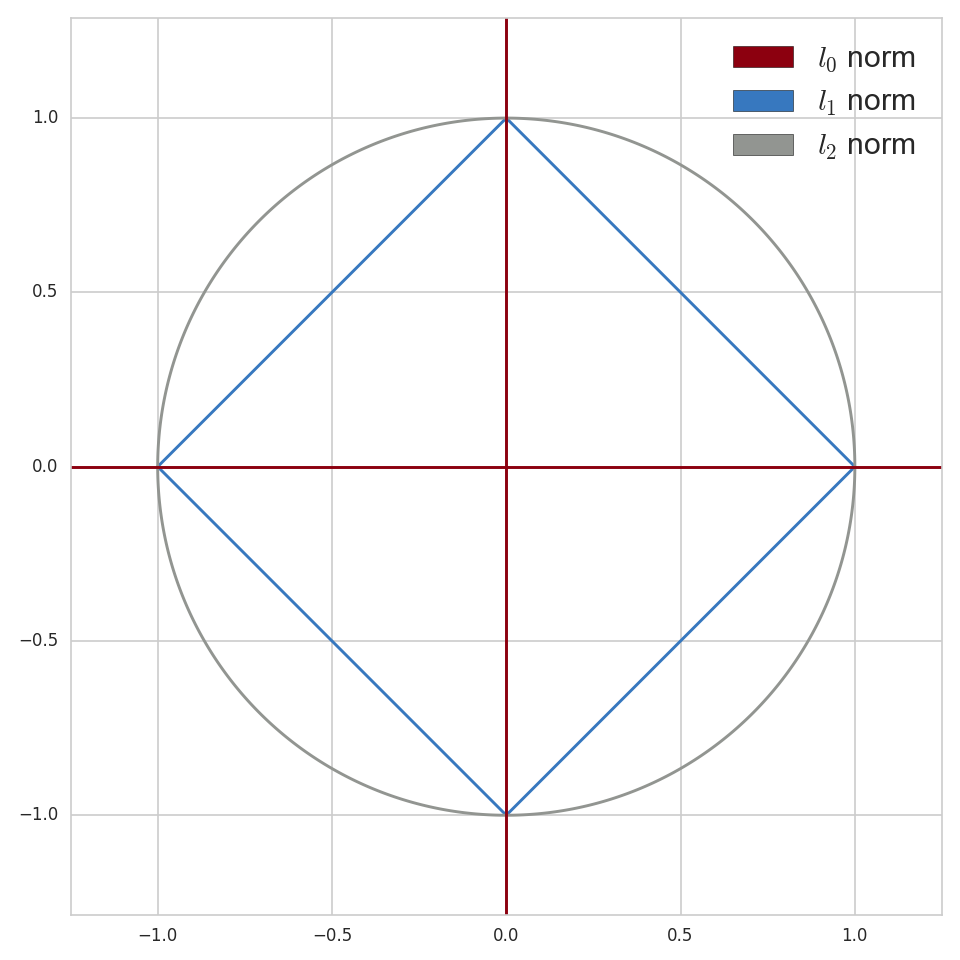
\includegraphics[scale=0.3]{img/l012_norms.png}
%\caption{contour plot of the $l_0, l_1, l_2$ norm at levelset $L_1(f) := \lbrace x \in \R^2 : f(x) = 1 \rbrace $. Note that for any space $\R^d$, the image of the $l_0$ consists of $d+1$ values ($\lbrace 0, ..., d \rbrace $).}
%\label{fig:l012plot}
%\end{figure}


%%%%%%%%%%%%%%
%%     Prior Work          %%
%%%%%%%%%%%%%%
\subsection{Related Work}\label{sec:prior-work}

In order to tackle the problem whose complexity mainly arises from the $\| .\|_0$ norm, one approach is to relax the norm to a more feasible one (i.e. LASSO, LARS for convex-relaxation or log penalty for non-convex relaxation). However, this might lead to over-penalization~\cite{nonconvexrelax}. Another ansatz is to utilize a greedy approach which constantly adds or removes variables based on some measure~\cite{submod_spectral}.  Another method attempts to adjust the dictionary and sparse representation in an online fashion~\cite{mairal09}. This can be stated as a maximization problem of a submodular function. A submodular function thereby can be viewed as a discrete analog to a convex function in the continuous case~\cite{submod_sparsecoding} which encodes the principle of ``diminishing returns". These submodular approximations to Sparse Dictionary Selection have become nearly ubiquitous in the literature with slight algorithmic variations that approach the theoretical bounds, $(1 - 1/e)$, set in~\cite{Krause05near-optimalnonmyopic}.
\\

\noindent Applications of Sparse Dictionary Learning---in particular the utilization of submodular approximations---are broad and varied; with uses found in classical Machine Learning (i.e. Sparse Linear Regression), Computer Vision(Image reconstruction, inpainting, denoising), Signal Processing~\cite{submod_sparsecoding}~\cite{nonconvexrelax}, Social Network Analysis, Statistics~\cite{rIBP}, and Economics~\cite{utilityWelfare} among many others. 
\\

\noindent There has been little work in Sparse Regression and Dictionary Learning that utilize the functional inverse of submodular approximations, known as supermodular functions. Supermodularity can facilitate the potential formulation of a dual to the native Dictionary Learning problem. Recently there has been some attempts at developing foundations for extending the suite of algorithms used in submodular maximization to supermodular formulations. In order to accomplish this, several caveats have been made on the functional representations themselves~\cite{weaklyalpha}. We leverage the gains made in submodular optimization and use recent results in approximating supermodular functions in constructing a two-stage supermodular minimization extension of the continuous greedy algorithm used in the submodular case~\cite{Singer16TwoStage}.

%%%%%%%%%%%%%%%
%%     Supermodularity     %%
%%%%%%%%%%%%%%%
\subsection{Supermodular Assumption}\label{sec:supermod}

\noindent Typical optimization problems that use submodular or supermodular functions are generally of the form:\\

\noindent Given a set of objects $V=\{v_1,\ldots,v_n\}$ and a function $f:2^V\to \R$ that returns a real value for any subset. Suppose we are interested in finding the subset that either maximizes or minimizes the function, e.g., ${arg\max}_{S\subseteq V} f(S)$, possible subject to some constraints on the size of $S$. In dictionary selection these constraints are generally on the number of iterms that the subset $S$ can contain, where the function encodes the accuracy of representing $V$ with $S$.

\noindent We begin by establishing key definitions and properties of sub-/supermodularity.\\

\noindent A function $f:2^V\to \R$ is \textit{submodular} if for any $A,\ B \subseteq V$ we have : $$f(A) + f(B) \geq f(A\cup B) + f(A\cap B)$$ An alternate and equivalent definition that aids in developing intuition is, in the event that $A\subseteq B \subseteq V$ and $v\in V\setminus B$ we have: $$f(A\cup \{v\}) - f(A) \geq f(B\cup\{v\}) - f(B)$$
This alternate definition of submodularity demonstrates a key feature of this class of functions; that is the marginal increase of any additional element diminishes with the overall size of the set. This is known as the ``diminishing returns" property of submodular functions.

\noindent Now, a function $f:2^V\to \R$ is said to be \textit{supermodular} if for any sets $A,\ B \subseteq V$ we have : $$f(A) + f(B) \leq f(A\cup B) + f(A\cap B)$$ This leads to a similar ``increasing returns" property given sets $A\subseteq B \subseteq V$ and $v\in V\setminus B$ we have: $$f(A\cup \{v\}) - f(A) \leq f(B\cup\{v\}) - f(B)$$

\noindent It is important to note that submodular and supermodular functions are inverses of each other. That relation motivates the excursion into the development of two-stage supermodular minimization, influenced by previous work in the development of similar methodology for submodular maximization.


%%%%%%%%%%%%%%%%%%%%%%%%%%%%%%%%%%%%%%%%%%%%%%%%%%%%
%%--------------------             Setting up the Analysis/Developing the Algorithm                --------------------%%
%%%%%%%%%%%%%%%%%%%%%%%%%%%%%%%%%%%%%%%%%%%%%%%%%%%%
\section{Evaluation}\label{sec:eval}

\subsection{Dictionary Selection as Two-Stage Supermodular Minimization} \label{supermodTwoStage}

In \cite{weaklyalpha}, the authors step through a few examples to demonstrate the application of supermodular functions to relevant problems. One that we highlight is that of Sparse Multiple Linear Regression (SMLR). We focus on this problem due to its close relation to Dictionary Selection (in fact we aim to show that these problems are functionally equivalent) as both problems are under the umbrella of Representation Learning. The goal of demonstrating the equivalence of SMLR and Dictionary Selection is that we can extend the theoretical guarantees and algorithmic foundations in~\cite{weaklyalpha} in our future work. 
\\

\noindent SMLR is defined as follows:\\
Given two matrices $X\in\R^{m\times n}$, $Y\in\R^{m\times l}$ and an integer $k$, find a matrix  $W\in\R^{n\times l}$ that minimizes $\|XW-Y\|^2_F$ subject to $W$ having at more $k$ non-zero rows. This problem is usually paired with a common assumption/simplification, where the columns of $X$ are adjusted to have unit norm.
\\

\noindent As outlined in Section~\ref{model}, here is a general definition of the Dictionary Selection problem.
\begin{alignat}{5}
         & \argmin_{\mathcal{D}, \mathcal{R}} \|X \ -&\mathcal{D}\mathcal{R}\|_F^2  + &\lambda \sum_{i=1}^k  \|\ r_i\|_0     \quad   \\
         &\text{s.t.}  \quad  &\|d_j\|_2 \leq 1&, \forall j=1, ...,n  \quad 
\end{alignat}
Thus, given an input dataset $X=[x_1, \dots, x_k], \ x_i\in\R^d, \ X\in\R^{d\times k}$ we wish to find the dictionary $\mathcal{D}\in\R^{d\times n}, \ \mathcal{D} = [d_1, \dots, d_n]$ and a representation $\mathcal{R}=[r_1,\dots,r_k], \ r_i\in\R^n, \ \mathcal{R}\in\R^{n\times k}$, such that both $\|X-\mathcal{D}\mathcal{R}\|_F^2$ is minimized and the representations $r_i$ are "sparse enough" (can be specified column by column as in \cite{rIBP}, or be extended as defined in SMLR).\\
\\
\noindent In SMLR, the data matrix $X$ with the determined, sparse $W$, are used to approximate $Y$ while in Dictionary Selection the matrices $\mathcal{D},\ \mathcal{R}$ are determined to approximate the data $X$. In both problems, sparse representations are used to select a combination of data that closely replicates known data. For all intents and purposes these two problems are functionally equivalent with consideration being made to ensure that the sparsity requirements of Dictionary Selection (where there is a limit on the sparsity of each row/column) port into those of SMLR (where the sparsity requirements are placed on the matrix in full). This isn't of too much concern as this can be handled in the definition of each specific application of the Dictionary Selection problem.\\
\\
Now, you'll note that the definition of the dictionary selection problem (Equation 6) requires the minimization over the matrices $\mathcal{D}\text{ and }\mathcal{R}$. When taken together, this problem is combinatorially infeasible~\cite{NPHardproof} and non-convex. However, if we separate the problem into a two-stage optimization (where we fix one matrix and solve for the other and then iterate) we can apply well understood convex solution strategies.~\cite{submod_spectral}, \cite{greedy_selection}, \cite{rIBP}, \cite{Singer16TwoStage}. These two stages are: 
\begin{enumerate}
\item Fix $\mathcal{D}$, find a sparse coding between it and $X$.
\item Solve the Dictionary Optimization problem: $\mathcal{D} = X\mathcal{R}^{+}$ following which we renormalize $\mathcal{D}$.
\end{enumerate}
Upon iteration we can expect convergence, using guarantees in the continuous greedy algorithm~\cite{greedy_selection}, \cite{submod_spectral}, \cite{submod_sparsecoding} as well as those made in \cite{weaklyalpha}. The commonly known sparse regression can be seen as an instance of sparse multiple linear regression with $Y$ existing only of one column. I.e. $XW-Y$ is a vector. 

\subsection{Weakly-$\alpha$ Supermodularity} \label{weakalpha}

Weakly-$\alpha$-supermodularity is a relaxation of supermodularity. With this relaxation, it can be shown that problems that are $\alpha$-weakly supermodular can be solved using a slightly adapted standard greedy algorithm. However, convergence typically requires more steps than  if the problem was supermodular only.
\\
\\
A non-negative, non-increasing set function $f(S): 2^{[n]} \rightarrow \mathbb{R}^+$ is weakly-$\alpha$-supermodular if there exists $\alpha \geq 1$ such that for any two sets $S, T \subseteq [n]$
\[f(S) - f(S \cup T) \leq \alpha \vert T \setminus S\vert \max_{i \in T \setminus S} f(S) - f(S \cup \lbrace i \rbrace) \]
To understand the definition better, assume we are given two disjoint sets $A, B \subseteq [n]$ with $A \cap B = \emptyset$. Then $\alpha$-weakly-supermodularity means that we can find an element $i \in B$ s.t. 
\[
\frac{f(A) - f(A \cup B)}{\alpha \vert B\vert} \leq f(A) - f(A \cup \lbrace i \rbrace)
\]
In words, we can find an element $i$ that is better (in terms of lowering the objective function) than $\frac{1}{\alpha}$ times the average gain of an element of $B$. Note that for a supermodular function $\alpha = 1$.
\\
\\
In order to solve the SMLR problem 
\[\min \lbrace f(S) : \vert S \vert \leq k \rbrace \]
for some $k$, the greedy extension algorithm needs at most 
\[ \left\lceil \alpha k \ln \left(f\left(\frac{S_0}{\epsilon}\right)\right)\right\rceil \]
 steps given a start solution $S_0$ (usually the empty set), a threshold error $\epsilon$ (i.e $f(S_k) \leq (1+\epsilon)f(S^*)$ for the optimal solution $S^*$) and the weakness-parameter $\alpha$ of the function $f$ \cite{weaklyalpha}.
 \\
 \\
As in \cite{weaklyalpha} the authors show that sparse regression can be seen as minimizing a $\alpha$-weakly supermodular function with $\alpha = \| X^+ \|_F$, the extended greedy algorithm presented can be used to solve sparse regression.


%%%%%%%%%%%%%%%%%%%%%%%%%%%%%%%%%%%%%%%%%%%%%%%%%%%%
%%----------------------------                                      Results                                      ---------------------------%%
%%%%%%%%%%%%%%%%%%%%%%%%%%%%%%%%%%%%%%%%%%%%%%%%%%%%
\section{Results}\label{sec:results}

HERE WE WILL TALK ABOUT THE RESULTS WE GET FROM LEOs EXCURSION INTO THE ANALYSIS


%%%%%%%%%%%%%%%%%%%%%%%%%%%%%%%%%%%%%%%%%%%%%%%%%%%%
%%----------------------------              Conclusion/Future Steps/Discussion                ---------------------------%%
%%%%%%%%%%%%%%%%%%%%%%%%%%%%%%%%%%%%%%%%%%%%%%%%%%%%
\section{Discussion}\label{sec:discuss}

Our primary next step is in taking measures to develop the structure for an extension of the continuous greedy algorithm from submodular functions. After developing this algorithm, which we intend to pattern after that done in~\cite{Singer16TwoStage}, we will need to develop guarantees for convergence, accuracy and efficiency. There are theoretical benchmarks that have been made in \cite{greedy_selection}, \cite{Krause05near-optimalnonmyopic} and \cite{nonconvexrelax} that we also need to be sure that we meet in the ``dual"-like formulation of supermodular optimization for dictionary selection. Once we have this algorithm in place we will need to apply it some data sets like those in ~\cite{Singer16TwoStage}.
\\
\\
In another step, we would like to implement the extended greedy algorithm presented in \cite{weaklyalpha} and compare its performance to other known approximative algorithms in order to better understand its limits or potential flaws. Eventually, this can also serve as a benchmark for the extension of the continuous greedy algorithm we seek to develop.

%%%%%%%%%%%%%%%%%%%%%%%%%%%%%%%%%%%%%%%%%%%%%%%%%%%%%
%%----------------------------                                    Past excerpts                                  ---------------------------%%
%%%%%%%%%%%%%%%%%%%%%%%%%%%%%%%%%%%%%%%%%%%%%%%%%%%%%
\section{Model/Problem Refocusing} \label{model}
We don't have any reason to refocus or redefine our project. There was initially some concern that our problem had already been solved in a satisfiable manner. We're happy to report that there is significant room for contribution in the realm of supermodular optimization. We began by developing intuition in supermodular and submodular optimization, highlighted here in this section, and by reviewing recent research in the development of algorithms for both supermodular minimization~\cite{weaklyalpha} and for a two-stage formulation of submodular maximization~\cite{Singer16TwoStage}. 




\section{Data}
So far, we haven't yet determined how we will use data to solidify our project as much of our work at this point is in understanding and developing the theory necessary to develop a new or modified algorithm. As we are looking to develop a novel algorithm to provide a new benchmark for approximate solutions to this class of problems, we will likely assimilate the data and experiments used in  \cite{submod_spectral}, \cite{greedy_selection}, \cite{rIBP}, \cite{Singer16TwoStage}, among others. 


\section{Completed Steps}

In our proposal we outlined the following course of action:
\begin{displayquote}
Our first step in this project will be to understand the supermodular minimzation framework in which sparse regression can be defined. Then, after having connected and identified sparse regression as supermodular minimization problem we want to show that dictionary selection is a 2-stage sparse regression. \\
\\
In the following step we need to understand the greedy algorithm for submodular maximization and its improvement, the continuous greedy algorithm. After this, understanding 2-stage submodular optimization would ideally allow us to connect the pieces, gain insight and finally propose a new algorithm of dealing with the problem.
\end{displayquote}

We have successfully completed the first of these stages (as will be shown in \ref{supermodTwoStage}) and are on our way toward completing the second.



\section{Next Steps}


\bibliographystyle{plain}
\bibliography{bibliography}

\end{document}